% ========================================
%	Header einbinden
% ========================================

\documentclass[bibtotoc,titlepage]{scrartcl}

% Deutsche Spracheinstellungen
\usepackage[ngerman,german]{babel, varioref}
\usepackage[T1]{fontenc}
\usepackage[utf8]{inputenc}

%\usepackage{marvosym}

\usepackage{amsfonts}
\usepackage{amssymb}
\usepackage{amsmath}
\usepackage{amscd}
\usepackage{amstext}
\usepackage{float}
\usepackage{caption}
\usepackage{wrapfig}
\usepackage{setspace}
\usepackage{threeparttable}
\usepackage{footnote}

\newfloat{formel}{htbp}{for}
\floatname{formel}{Formel}


\usepackage{longtable}

%\usepackage{bibgerm}

\usepackage{footnpag}

\usepackage{ifthen}                 %%% package for conditionals in TeX
\usepackage[amssymb]{SIunits}
%Fr textumflossene Bilder und Tablellen
%\usepackage{floatflt} - veraltet

%Fr Testzwecke aktivieren, zeigt labels und refs im Text an.
%\usepackage{showkeys}

% Abstand zwischen zwei Abs�zen nach DIN (1,5 Zeilen)
% \setlength{\parskip}{1.5ex plus0.5ex minus0.5ex}

% Einrckung am Anfang eines neuen Absatzes nach DIN (keine)
%\setlength{\parindent}{0pt}

% R�der definieren
% \setlength{\oddsidemargin}{0.3cm}
% \setlength{\textwidth}{15.6cm}

% bessere Bildunterschriften
%\usepackage[center]{caption2}


% Probleml�ungen beim Umgang mit Gleitumgebungen
\usepackage{float}

% Nummeriert bis zur Strukturstufe 3 (also <section>, <subsection> und <subsubsection>)
%\setcounter{secnumdepth}{3}

% Fhrt das Inhaltsverzeichnis bis zur Strukturstufe 3
%\setcounter{tocdepth}{3}

\usepackage{exscale}

\newenvironment{dsm} {\begin{displaymath}} {\end{displaymath}}
\newenvironment{vars} {\begin{center}\scriptsize} {\normalsize \end{center}}


\newcommand {\en} {\varepsilon_0}               % Epsilon-Null aus der Elektrodynamik
\newcommand {\lap} {\; \mathbf{\Delta}}         % Laplace-Operator
\newcommand {\R} { \mathbb{R} }                 % Menge der reellen Zahlen
\newcommand {\e} { \ \mathbf{e} }               % Eulersche Zahl
\renewcommand {\i} { \mathbf{i} }               % komplexe Zahl i
\newcommand {\N} { \mathbb{N} }                 % Menge der nat. Zahlen
\newcommand {\C} { \mathbb{C} }                 % Menge der kompl. Zahlen
\newcommand {\Z} { \mathbb{Z} }                 % Menge der kompl. Zahlen
\newcommand {\limi}[1]{\lim_{#1 \rightarrow \infty}} % Limes unendlich
\newcommand {\sumi}[1]{\sum_{#1=0}^\infty}
\newcommand {\rot} {\; \mathrm{rot} \,}         % Rotation
\newcommand {\grad} {\; \mathrm{grad} \,}       % Gradient
\newcommand {\dive} {\; \mathrm{div} \,}        % Divergenz
\newcommand {\dx} {\; \mathrm{d} }              % Differential d
\newcommand {\cotanh} {\; \mathrm{cotanh} \,}   %Cotangenshyperbolicus
\newcommand {\asinh} {\; \mathrm{areasinh} \,}  %Area-Sinus-Hyp.
\newcommand {\acosh} {\; \mathrm{areacosh} \,}  %Area-Cosinus-H.
\newcommand {\atanh} {\; \mathrm{areatanh} \,}  %Area Tangens-H.
\newcommand {\acoth} {\; \mathrm{areacoth} \,}  % Area-cotangens
\newcommand {\Sp} {\; \mathrm{Sp} \,}
\newcommand {\mbe} {\stackrel{\text{!}}{=}}     %Must Be Equal
\newcommand{\qed} { \hfill $\square$\\}
\renewcommand{\i} {\imath}
\def\captionsngerman{\def\figurename{\textbf{Abb.}}}

%%%%%%%%%%%%%%%%%%%%%%%%%%%%%%%%%%%%%%%%%%%%%%%%%%%%%%%%%%%%%%%%%%%%%%%%%%%%
% SWITCH FOR PDFLATEX or LATEX
%%%%%%%%%%%%%%%%%%%%%%%%%%%%%%%%%%%%%%%%%%%%%%%%%%%%%%%%%%%%%%%%%%%%%%%%%%%%
%%%
\ifx\pdfoutput\undefined %%%%%%%%%%%%%%%%%%%%%%%%%%%%%%%%%%%%%%%%% LATEX %%%
%%%
\usepackage[dvips]{graphicx}       %%% graphics for dvips
\DeclareGraphicsExtensions{.eps,.ps}   %%% standard extension for included graphics
\usepackage[ps2pdf]{thumbpdf}      %%% thumbnails for ps2pdf
\usepackage[ps2pdf,                %%% hyper-references for ps2pdf
bookmarks=true,%                   %%% generate bookmarks ...
bookmarksnumbered=true,%           %%% ... with numbers
hypertexnames=false,%              %%% needed for correct links to figures !!!
breaklinks=true,%                  %%% breaks lines, but links are very small
linkbordercolor={0 0 1},%          %%% blue frames around links
pdfborder={0 0 112.0}]{hyperref}%  %%% border-width of frames
%                                      will be multiplied with 0.009 by ps2pdf
%
\hypersetup{ pdfauthor   = {Hannes Franke; Julius Tilly},
pdftitle    = {V301 Innenwiderstand und Leistungsanpassung}, pdfsubject  = {Protokoll FP}, pdfkeywords = {V301, Innenwiderstand, Leistungsanpassung},
pdfcreator  = {LaTeX with hyperref package}, pdfproducer = {dvips
+ ps2pdf} }
%%%
\else %%%%%%%%%%%%%%%%%%%%%%%%%%%%%%%%%%%%%%%%%%%%%%%%%%%%%%%%%% PDFLATEX %%%
%%%
\usepackage[pdftex]{graphicx}      %%% graphics for pdfLaTeX
\DeclareGraphicsExtensions{.pdf}   %%% standard extension for included graphics
\usepackage[pdftex]{thumbpdf}      %%% thumbnails for pdflatex
\usepackage[pdftex,                %%% hyper-references for pdflatex
bookmarks=true,%                   %%% generate bookmarks ...
bookmarksnumbered=true,%           %%% ... with numbers
hypertexnames=false,%              %%% needed for correct links to figures !!!
breaklinks=true,%                  %%% break links if exceeding a single line
linkbordercolor={0 0 1},
linktocpage]{hyperref} %%% blue frames around links
%                                  %%% pdfborder={0 0 1} is the default
\hypersetup{
pdftitle    = {V301 Innenwiderstand und Leistungsanpassung}, 
pdfsubject  = {Protokoll AP}, 
pdfkeywords = {V301, Innenwiderstand, Leistungsanpassung},
pdfsubject  = {Protokoll AP},
pdfkeywords = {V301, Innenwiderstand, Leistungsanpassung}}
%                                  %%% pdfcreator, pdfproducer,
%                                      and CreationDate are automatically set
%                                      by pdflatex !!!
\pdfadjustspacing=1                %%% force LaTeX-like character spacing
\usepackage{epstopdf}
%
\fi %%%%%%%%%%%%%%%%%%%%%%%%%%%%%%%%%%%%%%%%%%%%%%%%%%% END OF CONDITION %%%
%%%%%%%%%%%%%%%%%%%%%%%%%%%%%%%%%%%%%%%%%%%%%%%%%%%%%%%%%%%%%%%%%%%%%%%%%%%%
% seitliche Tabellen und Abbildungen
%\usepackage{rotating}
\usepackage{ae}
\usepackage{
  array,
  booktabs,
  dcolumn
}
\makeatletter 
  \renewenvironment{figure}[1][] {% 
    \ifthenelse{\equal{#1}{}}{% 
      \@float{figure} 
    }{% 
      \@float{figure}[#1]% 
    }% 
    \centering 
  }{% 
    \end@float 
  } 
  \makeatother 


  \makeatletter 
  \renewenvironment{table}[1][] {% 
    \ifthenelse{\equal{#1}{}}{% 
      \@float{table} 
    }{% 
      \@float{table}[#1]% 
    }% 
    \centering 
  }{% 
    \end@float 
  } 
  \makeatother 
%\usepackage{listings}
%\lstloadlanguages{[Visual]Basic}
%\allowdisplaybreaks[1]
%\usepackage{hycap}
%\usepackage{fancyunits}

% ========================================
%	Angaben für das Titelblatt
% ========================================

\title{Versuch 27 - Der Zeeman-Effekt\\				% Titel des Versuchs 
\large TU Dortmund, Fakultät Physik\\ 
\normalsize Fortgeschrittenen-Praktikum}

\author{Jan Adam\\			% Name Praktikumspartner A
{\small \href{jan.adam@tu-dortmund.de}{jan.adam@tu-dortmund.de}}	% Erzeugt interaktiven einen Link
\and						% um einen weiteren Author hinzuzfügen
Dimitrios Skodras\\					% Name Praktikumspartner B
{\small \href{dimitrios.skodras@tu-dortmund.de}{dimitrios.skodras@tu-dortmund.de}}		% Erzeugt interaktiven einen Link
}
\date{07. März 2014}				% Das Datum der Versuchsdurchführung

% ========================================
%	Das Dokument beginnt
% ========================================

\begin{document}

% ========================================
%	Titelblatt erzeugen
% ========================================

\maketitle					% Jetzt wird die Titelseite erzeugt
\thispagestyle{empty} 				% Weder Kopfzeile noch Fußzeile

% ========================================
%	Der Vorspann
% ========================================

%\newpage					% Wenn Verzeichnisse auf einer neuen Seite beginnen sollen
%\pagestyle{empty}				% Weder Kopf- noch Fußzeile für Verzeichnisse

\tableofcontents

%\newpage					% eine neue Seite
%\thispagestyle{empty}				% Weder Kopf- noch Fußzeile für Verzeichnisse
%\listoffigures					% Abbildungsverzeichnis

%\newpage					% eine neue Seite
%\thispagestyle{empty}				% Weder Kopf- noch Fußzeile für Verzeichnisse
%\listoftables					% Tabellenverzeichnis
\newpage					% eine neue Seite


% ========================================
%	Kapitel
% ========================================

%\section{Einleitung}				% Bei Bedarf

\section{Theorie}
\setcounter{page}{1}
Der Zeeman-Effekt ist ein Phänomen, bei dem Energieniveaus von Hüllenelektronen, die in der Orientierungsquantenzahl $m$ entartet sind, in Gegenwart eines
äußeren, homogenen Magnetfelds aufgespalten werden. Ziel des Versuchs ist es, Größe und Anzahl dieser Aufspaltung zu ermitteln.
\subsection{Drehimpulse und Magnetische Momente}
\label{sec_Jmu}
Die Ursache des Effekts hängt mit den Drehimpulsen - Bahndrehimpuls $\vec l$ und Spin $\vec s$ - der Elektronen und den daraus resultierenden 
magnetischen Momenten zusammen. Die Lösung der Eigenwertgleichung liefert für die Drehimpulse folgende Werte, wobei $\hbar$ das Plancksche Wirkungsquantum
und $n$ die Hauptquantenzahl ist
\begin{align}
 \left|\vec l\right| &= \sqrt{l(l+1)}\hbar \hspace{1cm} \text{mit } l=0,1,..,n-1\\
 \left|\vec s\right| &= \sqrt{s(s+1)}\hbar \hspace{0.9cm} \text{mit } s=\frac12
\end{align}
Das auf die die Drehimpulseinheit $\hbar$ bezogene Magnetmoment ist das Bohrsche Magneton
\begin{align}
 \mu_B = -\frac12\frac{e_0\,\hbar}{m_0},
\end{align}
mit $e_0$ als Elementarladung und $m_0$ als Elektronenmasse. Aus $\mu_B$ lässt sich das $\vec l$ zugehörige magnetische Moment bestimmen zu
\begin{align}
 \vec \mu_l = -\mu_B \frac{\vec l}{\hbar} = -\mu_B\sqrt{l(l+1)}\, \textbf{e}_l.
\end{align}
Da der Spin auch ein Drehimpuls ist, liegt der Schluss nahe, dass dieser auch ein magnetisches Moment besitzt
\begin{align}
 \vec \mu_s = -g_s \mu_B \frac{\vec s}{\hbar} = -g_s \mu_B \sqrt{s(s+1)}\, \textbf{e}_s
\end{align}
Der Landé-Faktor des Elektrons $g_s$ hat etwa den Wert 2 und führt zu einem doppelt so großen Wert für das magnetische Moment, wie das dem Bahndrehimpuls
zugehörige magnetische Moment. Das wird magnetomechanische Anomalie des Elektrons genannt.

Die bisher genannten Zusammenhänge beziehen sich auf Einelektronsysteme und betrachten keine Wechselwirkung zwischen Spin und Bahndrehimpuls. Bei
mehreren Elektronen und allgemeiner Betrachtung entstehen sehr komplexe Zusammenhänge. Daher werden nur zwei Grenzfälle betrachtet, deren Behandlung
einfach ist. Bei geringen Kernladungszahlen $Z$ führt die hohe Wechselwirkung der einzelnen Bahndrehimpulse $\vec l_i$ zu einem Gesamtbahndrehimpuls $\vec L$
und einem zugehörigen magnetischen Moment.
\begin{align}
 \vec L = \sum_i \vec l_i\hspace{1cm} \text{mit } L=0,1,2,3
\end{align}
Hierzu müssen nur unabgeschlossene Schalen berücksichtigt werden, da Gesamtdrehimpulse abgeschlossener Schalen stets null sind. Analog zum Gesamtbahndrehimpuls
lässt sich ein Gesamtspin $\vec S$ bestimmen, mit $N$ als Gesamtzahl der Elektronen auf nichtabgeschlossenen Schalen
\begin{align}
 \vec S = \sum_i \vec s_i\hspace{1cm} \text{mit } S=\frac{N}{2}, \frac{N}{2}-1,..., \frac12,0
\end{align}
In Abwesenheit starker Magnetfelder addieren Gesamtbahndrehimpuls und Gesamtspin zum Gesamtdrehimpuls $\vec J$, was LS-Kopplung oder Russel-Sauners-Kopplung
bezeichnet wird.
\begin{align}
 \vec J = \vec L = \vec S
 \label{eq_JLS}
\end{align}

Der zweite Grenzfall beschreibt die Wechselwirkung bei hohen Kernladungszahlen und wird j-j-Kopplung genannt. Hier ist die Kopplung von $\vec l$
und $\vec s$ eines einzelnen Elektrons entscheidender, als die Wechselwirkungen der Drehimpulse mit ihren Äquivalenten anderer Elektronen. Entsprechend
bildet sich der Gesamtdrehimpuls $\vec J$ nicht aus summierten Spin und Bahndrehimpuls, sondern aus den einzelnen Gesamtdrehimpulsen $\vec j_i$ der einzelnen
Elektronen selbst
\begin{align}
 \vec J = \sum_i \vec j_i.
\end{align}
Zwischen den Grenzfällen großer und kleiner Ordnungszahlen besteht ein fließender Übergang. Das $\vec J$ zugehörige magnetische Moment $\mu_j$ 
wird wie $\vec J$ nach \eqref{eq_JLS} selbst aus Spin und Bahndrehimpuls errechnet
\begin{align}
 \vec \mu_j = \vec \mu_s + \vec \mu_l.
 \label{eq_mujls}
\end{align}
Da $\vec J$ nicht zwingend parallel zu $\vec \mu_j$ ist, kann man sich einen parallelen und senkrechten Teil von $\vec \mu_j$ generieren. Die 
senkrechte Komponente wird dabei null, was unter klassischer Betrachtung einer Präzession um die von außen vorgegebene Richtung gleich kommt, 
die im zeitlichen Mittel verschwindet. In \eqref{eq_mujls} die magnetischen Momente eingesetzt führt zu folgender Form
\begin{align}
 \vec \mu_J \approx \mu_B\sqrt{J(J+1)}\underbrace{\frac{3J(J+1+S(S+1)-L(L+1)}{2J(J+1)}}_{g_J} = \mu_B\sqrt{J(J+1)} \,g_J ,
 \label{eq_lande}
\end{align}
mit $g_J$ als Landé-Faktor des betreffenden Atoms.

Die im Weiteren benötigte Richtungsquantelung ist ein quantenmechanisches Phänomen, das nur Winkel zwischen $\mu_J$ und einem äußeren Magnetfeld
$\vec B = B \textbf{e}_z$ auftreten können, wenn die Parallelkomponente ein ganzzahliges Vielfaches von $g_J\mu_B$ ist
\begin{align}
 \mu_{J_z} = -m g_J\mu_B,
\end{align}
mit $m$ als eingangs erwähnte Orientierungsquantenzahl, deren Wert sich ganzzahlig nur zwischen $-J$ und $J$ bewegen kann. 
\subsection{Aufspaltung von Energieniveaus bei homogenem Magnetfeld}
Mit der Vorarbeit aus Abschnitt \ref{sec_Jmu} ist man nun in der Lage, die Zusatzenergie $E_{\text{mag}}$ zu berechnen, die ein Moment $\vec \mu$
im äußeren Magnetfeld $\vec B$ hinzugewinnt. Allgemein lässt sich sagen, dass
\begin{align}
 E_{\text{mag}} = -\vec \mu_J \circ \vec B = mg_J\mu_B B.
\end{align}
Hieran sieht man, dass für $B\neq0$ das Energieniveau $E_0$ in $2J+1$ äquidistante Niveaus auf, wie in Abbildung \ref{pic_Eniv}
\begin{figure}[H]
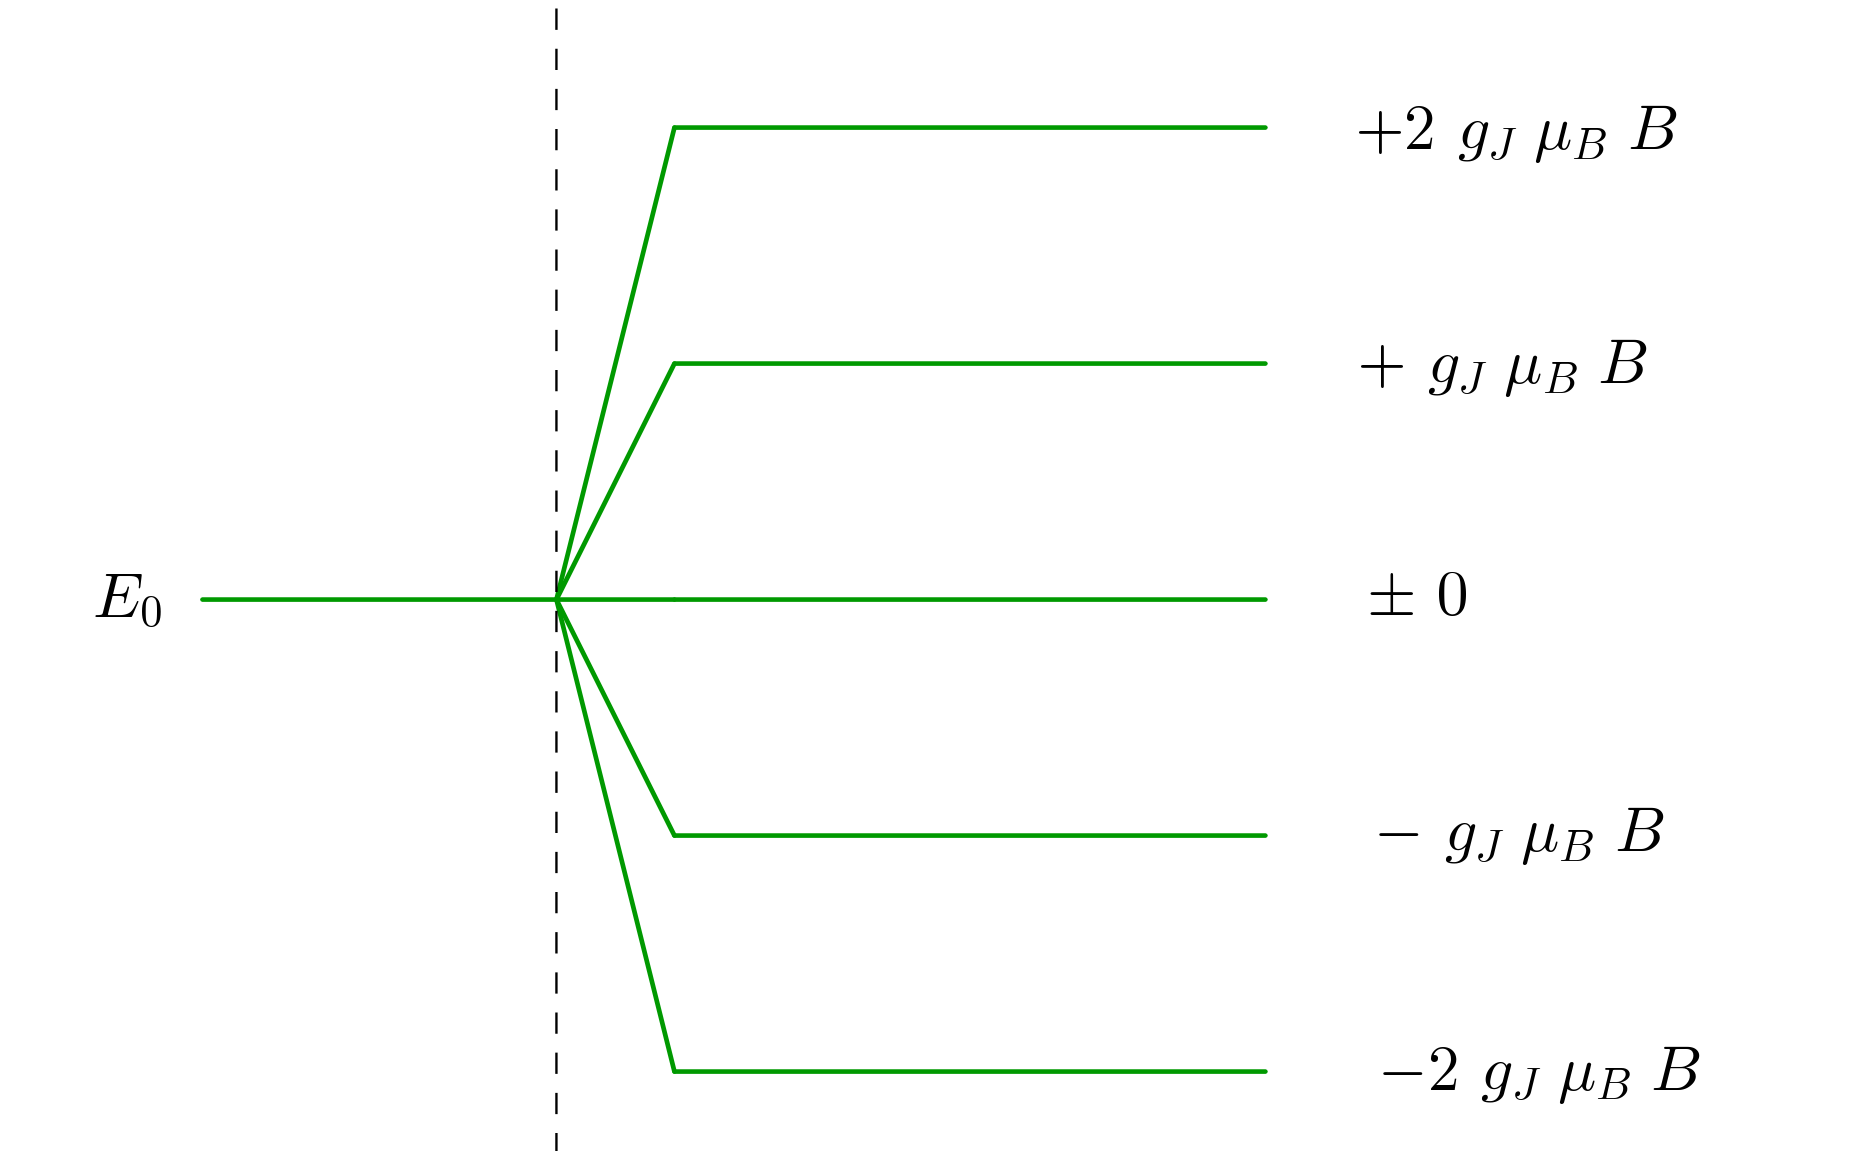
\includegraphics[width=0.7\textwidth]{../pics/Zeeman.png}
\caption{Schematische Aufspaltung eines Energieniveaus im Magnetfeld mit $J$ = 2}
\label{pic_Eniv}
\end{figure}
Zwischen den hinzukommenden Energieniveaus ist es nun möglich, dass Übergänge auftreten. Dieser Effekt wird als Zeeman-Effekt bezeichnet.
Die Anzahl dieser Linien hängt davon ab, welche Übergänge überhaupt möglich sind, ob es also Auswahlregeln gibt, die den Übergang festlegen.

Um sie zu ermitteln, wird die zeitabhängige Schrödingergleichung
\begin{align}
 \text{i}\hbar \frac{\partial}{\partial t}\psi(\vec r, t) = \left(-\frac{\hbar^2}{2m}\Delta + V\right) \psi(\vec r,t)
 \label{eq_schroedinger}
\end{align}
mit den Lösungen
\begin{align}
 \psi_1 (\vec r, t) = \psi_1(\vec r) \exp(-\text{i}\frac{E_\alpha}{\hbar}t)
\end{align}
betrachtet, mit $\Delta$ als Laplace-Operator, $V$ als ein Potenzial, $E_i$ als Energieeigenwert und $\psi_i(\vec r,t)$ als Wellenfunktion, die
von den Quantenzahlen $n_i, l_i$ und $m_i$ abhängt. Eine weitere Lösung von \eqref{eq_schroedinger} $\psi_2(\vec r,t)$ mit entsprechenden Quantenzahlen
soll existieren. Beide Lösungen bilden eine Linearkombination
\begin{align}
 \Psi(\vec r,t) = C_1\psi_1(\vec r,t) + C_2 \psi_2(\vec r,t),
\end{align}
die ebenfalls eine Lösungen der Schrödingergleichung ist und $C_i \in \mathbb{C}$. Aus der Berechnung der zeitabhängigen Dichteverteilung 
$\rho=\int\Psi^{*} \Psi \dx V$ ergibt sich, dass sie Schwingungen von Elektronen mit der Frequenz
\begin{align}
 \nu_{12} = \frac{E_1-E_2}{h}
\end{align}
beschreibt. Die damit verbundene Strahlungsintensität fordert ein Dipolmoment des schwingendne Elektrons, welches Komponenten in alle Raumrichtungen
hat. Diese berechnen sich zu
\begin{align}
 D_\alpha = -e_0 \int \alpha \Psi^*\Psi \dx V \hspace{1cm} \text{mit } \alpha = x,y,z.
\end{align}
Hier wird die Komponente $\alpha$ eines beliebig orientierten Dipols mit Frequenz $\nu_{12}$ beschrieben. Die hierin auftretenden Ausdrücke
\begin{align}
 \alpha_{12} = \int \alpha \psi_1^*\psi_2
 \label{eq_matrixelements}
\end{align}
werden Matrixelemente genannt, die für die Berechnung der Strahlungsintensität über den Poynting-Vektor $\vec S_{12}$ entscheidend sind
\begin{align}
\left| \vec S_{12}\right| \sim \left[\sum_\alpha\left| \alpha_{12}\right|\right]\sin^2\gamma.
\label{eq_poynting}
\end{align}
Errechnet werden die Elemente durch den kugelsymmetrischen Ansatz der Wellenfunktionen und die Tranformation in Kugelkoordinaten
\begin{align}
 \Psi = \frac{1}{\sqrt{2}}R(r)\Theta(\vartheta)\e^{\text{i}m\varphi} \hspace{1cm}\begin{pmatrix} x \\ y\\z \end{pmatrix}=r\begin{pmatrix}\cos\varphi\sin\vartheta \\ \sin\varphi\sin\vartheta \\ \cos\vartheta \end{pmatrix}
\end{align}
Nach Einsetzen in \eqref{eq_matrixelements} folgen die Auswahlregeln
\begin{align}
 m_2 = m_1, \hspace{0.5cm} m_2 = m_1\pm1
\end{align}
Folglich gibt es drei Konfigurationen, bei denen ein Übergang auftreten kann. Nun werden die Eigenschaften dieser Übergänge untersucht. Für 
$\Delta m = 0$  ist die Richtung des Dipols parallel zur Magnetfeldrichtung. Die Winkelabhängigkeit aus \eqref{eq_poynting} bedingt, dass nicht
in Feldrichtung abgestrahlt wird. Die Emission ist senkrecht zum Magnetfeld maximal, was bedeutet, dass diese Strahlung zu $\vec B$ parallel 
linear polarisiert ist. Betrachtungen von $\Delta m = \pm 1$ beschreiben um die Magnetfeldrichtung zirkularpolarisierte Schwingung mit jeweiliger
Drehrichtung.

\subsection{normaler und anormaler Zeeman-Effekt}                  
Die Einschränkung, dass \eqref{eq_schroedinger} nicht den Elektronenspin enthält, bedingt, dass die Ergebnisse nur für den Spezialfall $S=0$ gelten.
Dies nennt man den normalen Zeeman-Effekt. Es folgt, dass $g_J$ nach \eqref{eq_lande} 1 für alle J ist und daher von den Quantenzahlen unabhängig ist
Daher gilt für die Verschiebung der Energieniveaus
\begin{align}
 \Delta E = m \mu_B B \hspace{1cm} \text{mit } -J \leq m \leq J.
\end{align}
Wie man Abbildung \ref{pic_norZee} entnehmen kann, sind effektiv nur drei Linien zu beobachten. Übergänge mit gleichem $\Delta m$ sind energetisch
identisch.
\begin{figure}[H]
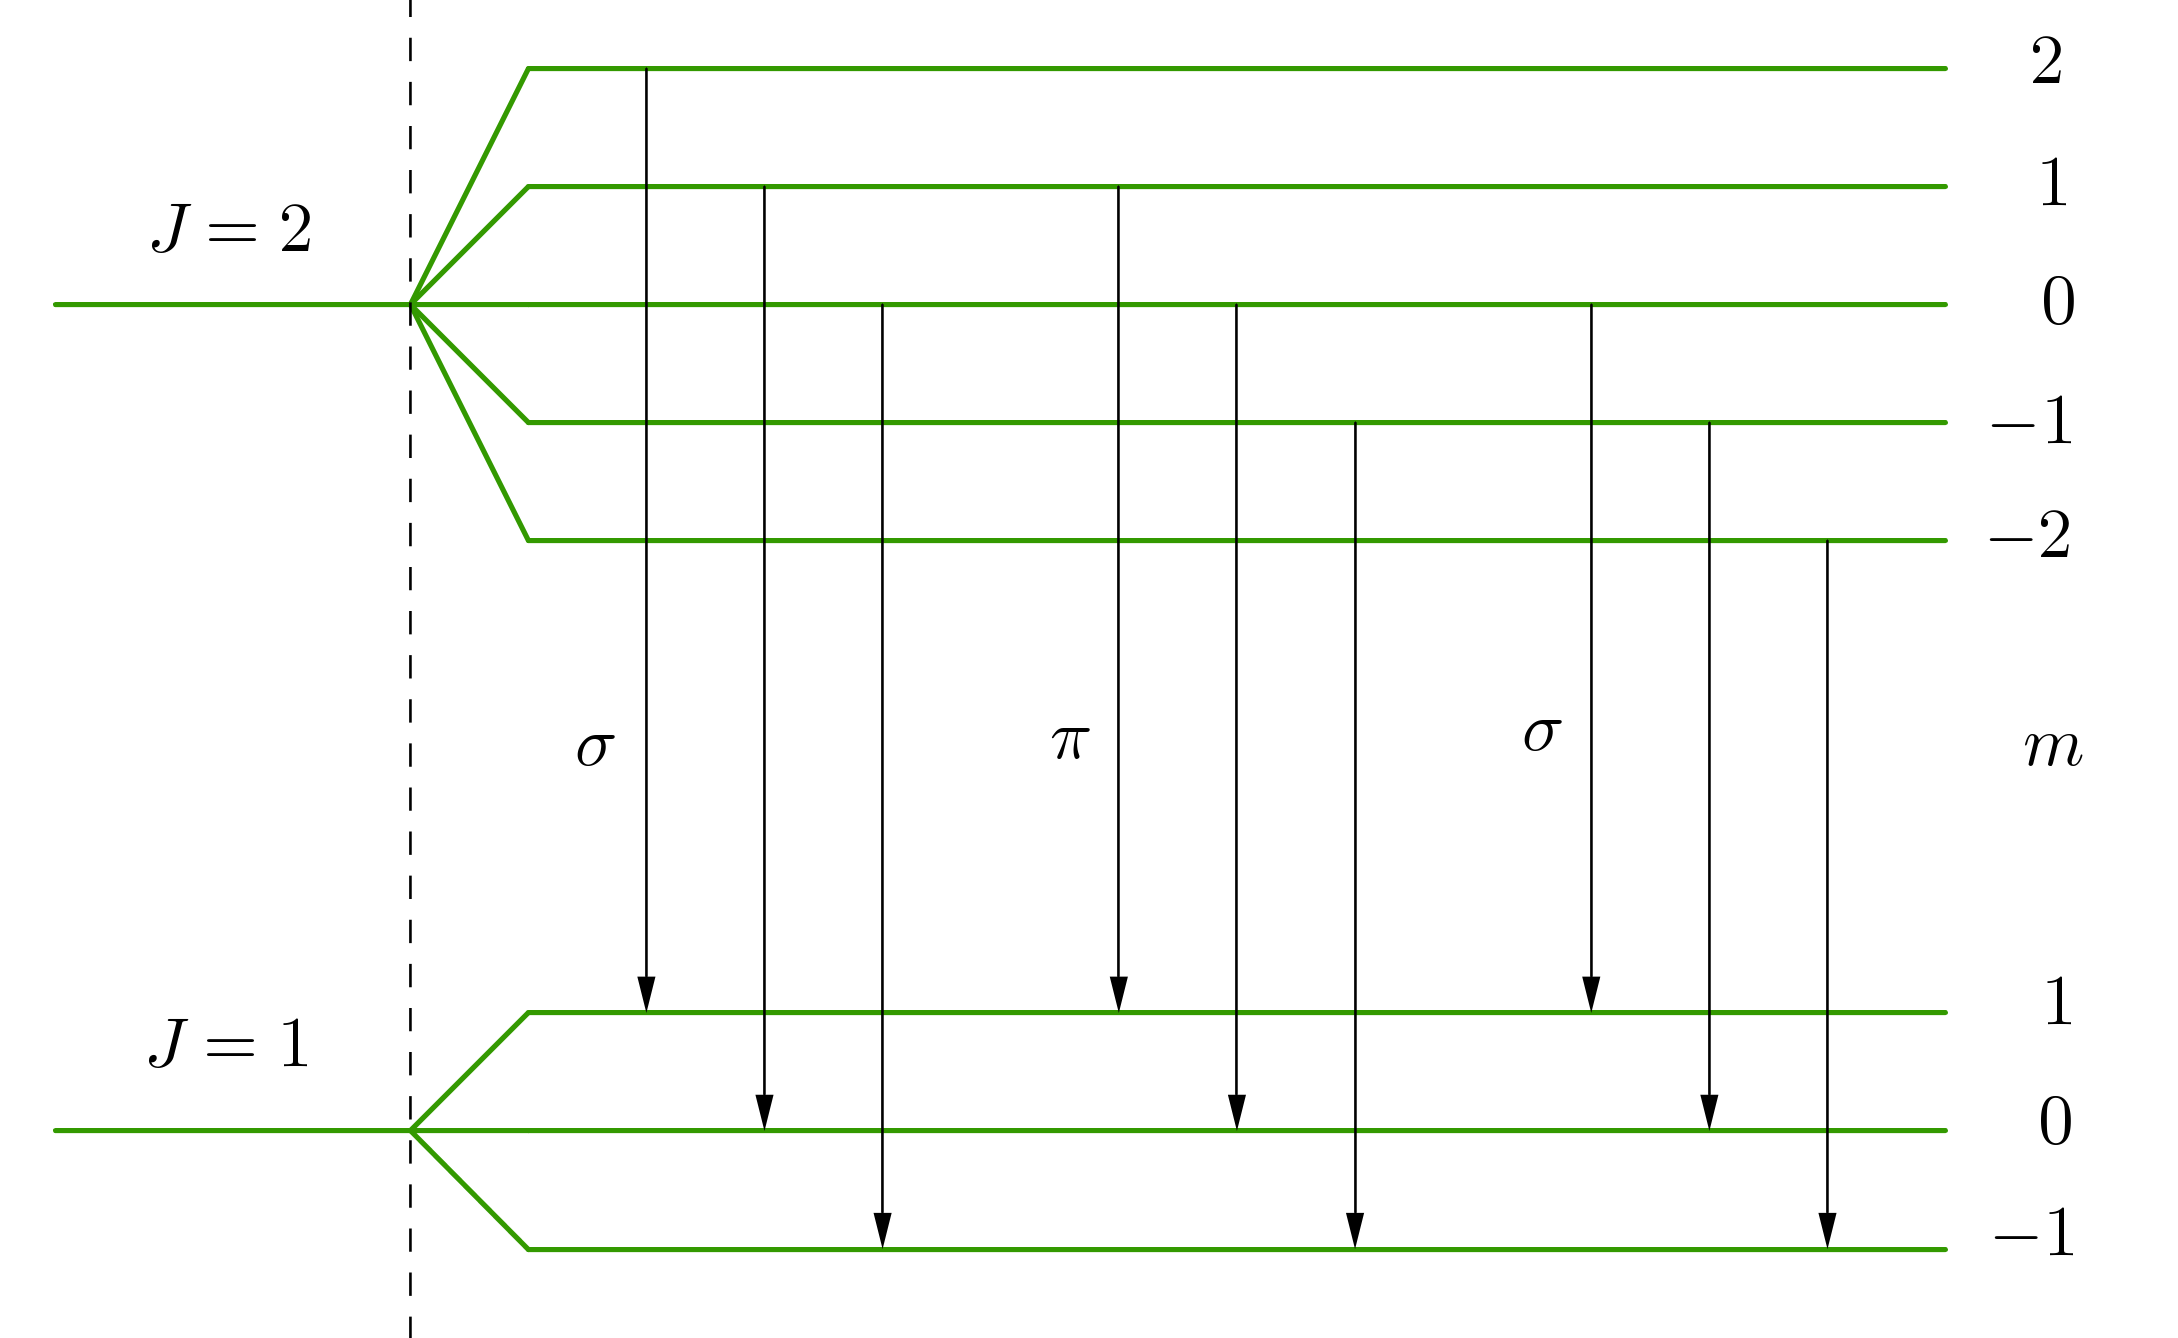
\includegraphics[width=0.7\textwidth]{../pics/norZee.png}
\caption{Aufspaltung und Polarisation beim Normalen Zeemaneffekt}
\label{pic_norZee}
\end{figure}
Die Polarisation bedingt, dass die emittierte Strahlung nicht in allen Beobachtungsrichtungen erkannt wird. Übergänge mit $\Delta m$ haben im Vergleich
zum Fall ohne ein Magnetfeld keine Energieänderung. Daher ist wie bereits gezeigt linear polarisiert und wird $\pi$-Komponente bezeichnet. Sie wird
daher nur transversal zur Feldrichtung beobachtet. Die anderen beiden Komponenten werden mit $\sigma$ bezeichnet und sind zirkular polarisiert und 
erscheinen bei transversaler Beobachtung linear polarisiert.

Der verallgemeinerte Zeeman-Effekt ist der mit $S\neq0$ und wird anormaler Zeeman-Effekt genannt. Aus der spinabhängigen Schrödingergleichung ergeben
sich dieselben Auswahlregeln. Relativ zur feldfreien Energie ergibt sich hier bei Übergängen zwischen zwei Niveaus folgende Energiedifferenz
\begin{align}
 \Delta E = [m_1 g(L_1,S_1,J_1)\, - \,m_2g(L_2,S_2,J_2)]\mu B
\end{align}
Der Landé-Faktor hängt hier von den Drehimpulsen ab, sodass die Aufspaltung linienreicher wird, was beispielhaft an einem Alkali-Dublett in Abbildung
\ref{pic_anorZee} dargestellt ist.
\begin{figure}[H]
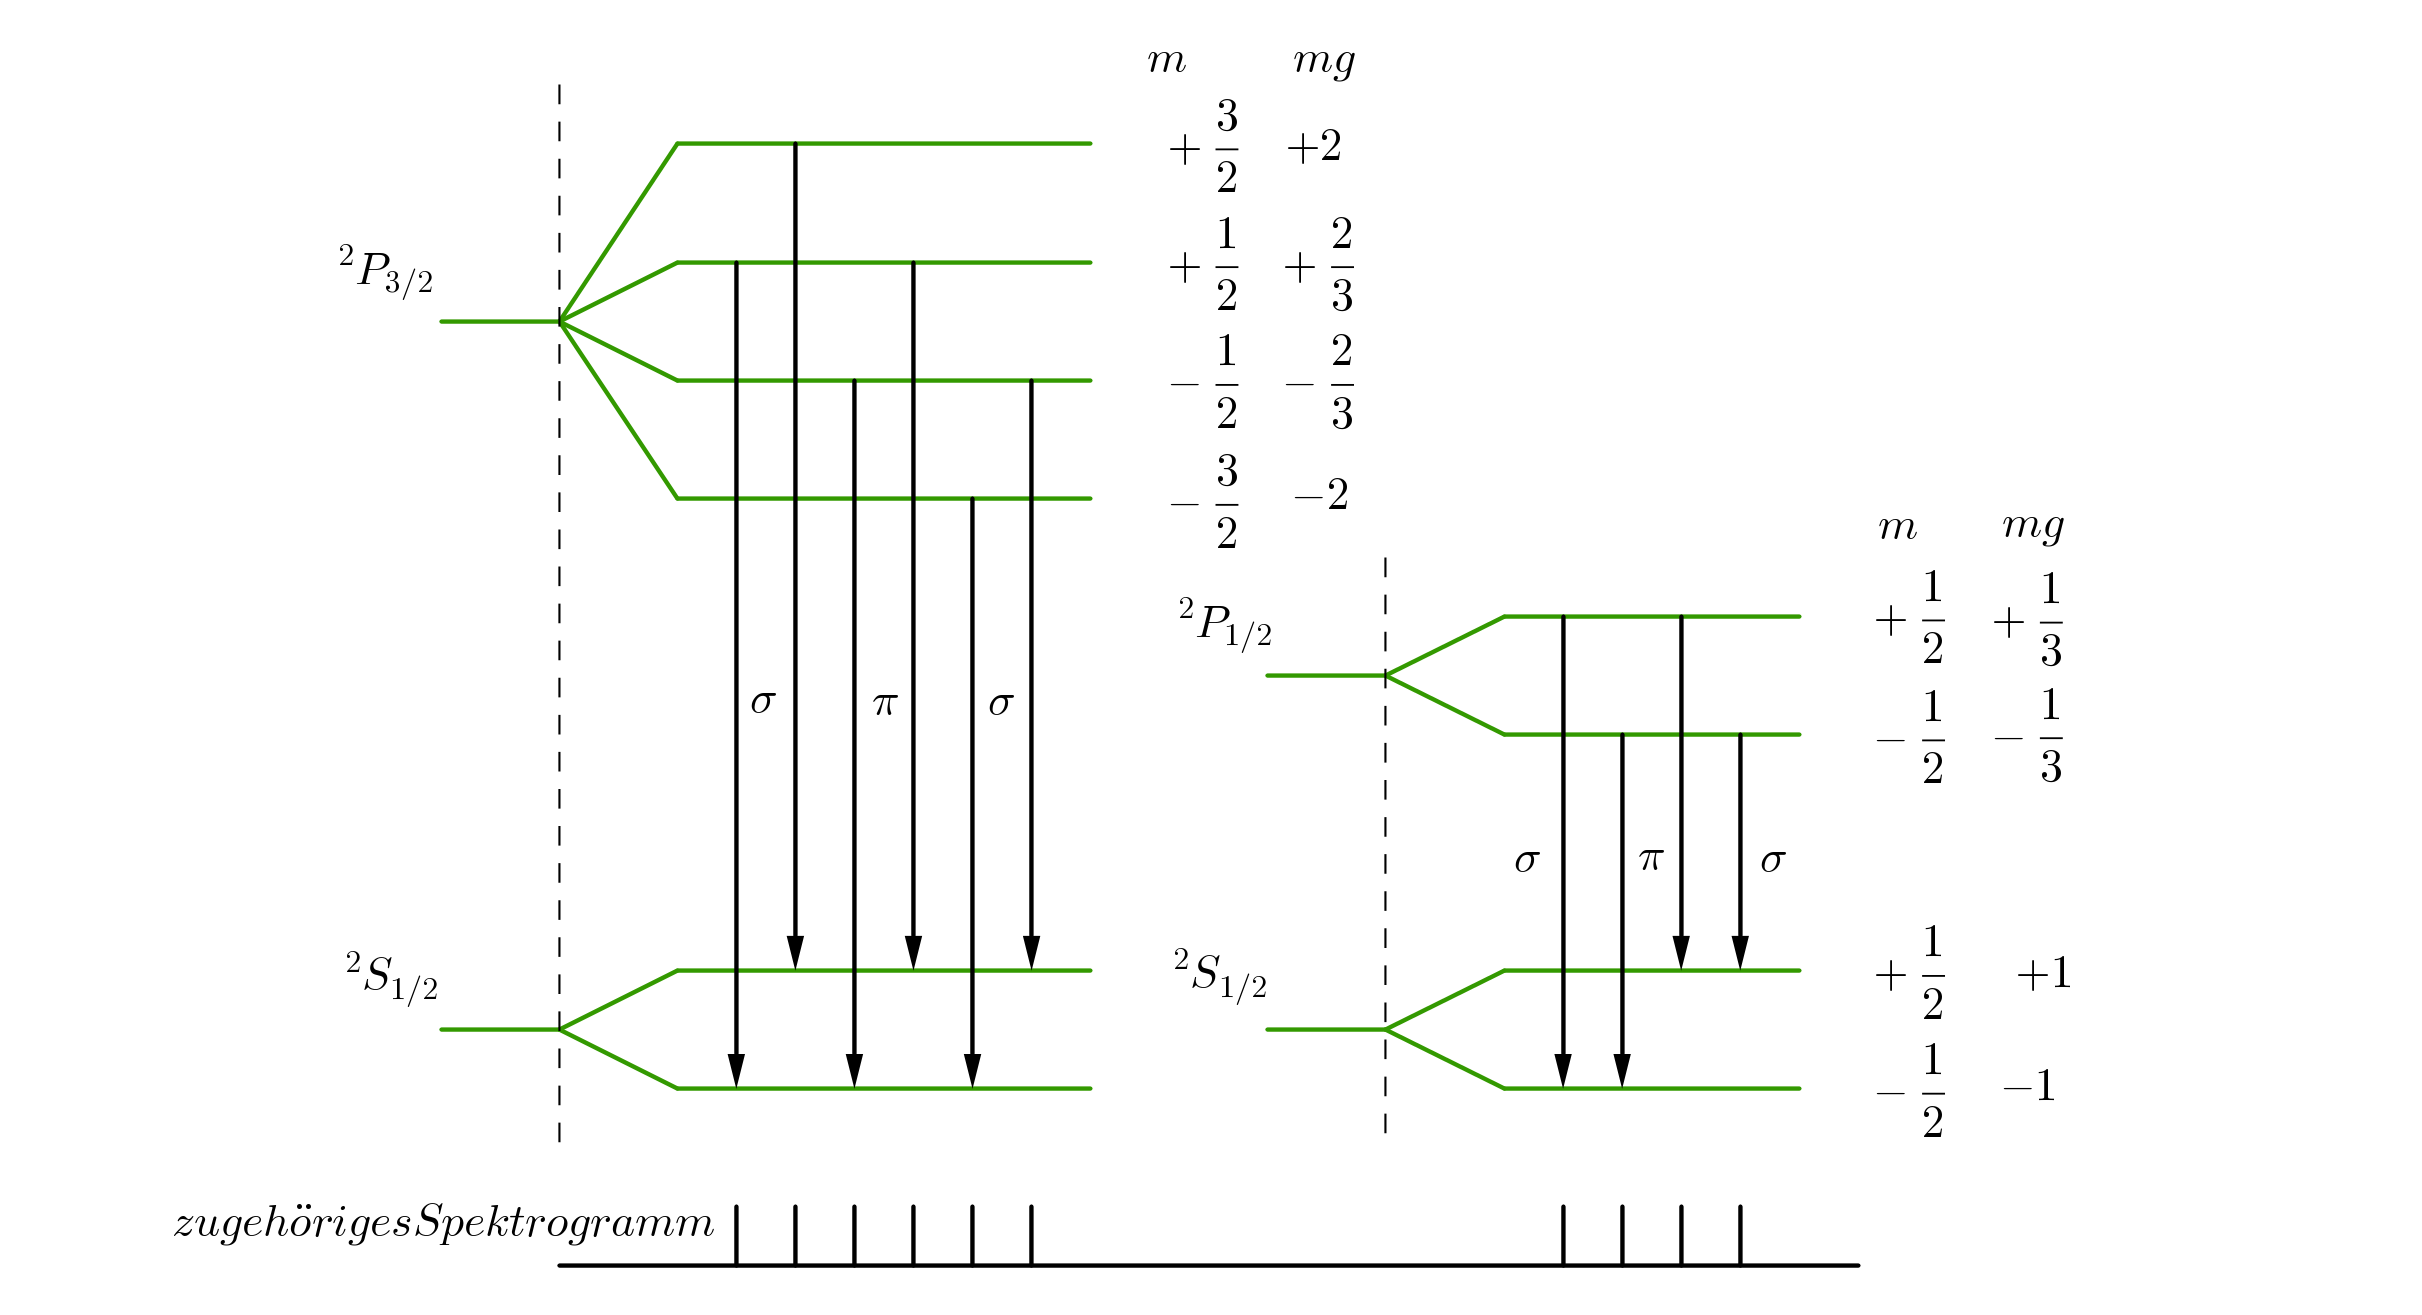
\includegraphics[width=1\textwidth]{../pics/anorZee.png}
\caption{Aufspaltung und Polarisation beim Anormalen Zeemaneffekt}
\label{pic_anorZee}
\end{figure}

\section{Durchführung}
bla
\section{Auswertung}

\parskip 340pt
\Large{Literatur}\\\\

% ========================================
%	Literaturverzeichnis
% ========================================

%\bibliographystyle{plainnat}			% Bibliographie-Style auswählen
%\bibliography{BIBDATEI}			% Literaturverzeichnis

% ========================================
%	Das Dokument endent
% ========================================

\end{document}
